\section{Protocolo de comunicación}
Como se estudió en el marco teórico, en una arquitectura
de comunicación, el protocolo CAN trabaja en las
capas inferiores del modelo de OSI. CAN propone cómo debe ser
el medio físico, y la manera de transmisión de las señales.
Además, preve cuál es la estrategia a utilizar  para sincronizar
la transmisión de datos sin nigún tipo de latencia, ni tampoco
colisiones de mensajes. Así, este protocolo permite que estos
sean enviados teniendo en cuenta sus prioridades, eliminando las colisiones, y
por lo tanto también, el tiempo de espera en la que los nodos se quedan
relegados cuando han tratado de enviar un mensaje al mismo tiempo.

Este protocolo no establece nada sobre ruteos de mensajes, tipos de mensajes y
tipos de datos, que a la hora de desarrollar una arquitectura de aviónica es
importante tener en cuenta esos detalles. Es necesario, que exista una
capa de servicios que facilite la comunicación entre aplicaciones de usuarios
de diferentes nodos, y la comunicación entre las aplicaciones de usuario
y el protocolo CAN (de bajo nivel) en sí.
Además, teniendo en cuenta los resultados obtenidos en las secciones
anteriores, se necesita, diseñar un protocolo de comunicación
basado en redes distribuidas, y que a su vez, esté basado en CAN.

Por tales motivos, surge la necesidad
de diseñar un protocolo de comunicación basado en CAN, que se ``monte'' sobre
las capas superiores del modelo de referencia de OSI; y que permita
la distribución de las tareas y el procesamiento llevado a cabo
por los nodos. 

El protocolo CANae se encuentra en su primera versión 0.1 Alpha. Esto hace
referencia a que en esta instancia de trabajo se trata de comprender
el problema y llevar a cabo un diseño preliminar del protocolo. De esta
manera se podrá extraer, tanto puntos positivos, como puntos negativos; o
más bien fortalezas y debilidades del stack de servicios que brinda CANae.

CANae actúa en la capa de aplicación del modelo de referencia de OSI. CANae
divide esta capa en dos subcapas:
\begin{itemize}
\item CANae Application Layer
\item CANae High Application layer
\end{itemize}

\begin{figure}[h!]
 \centering
 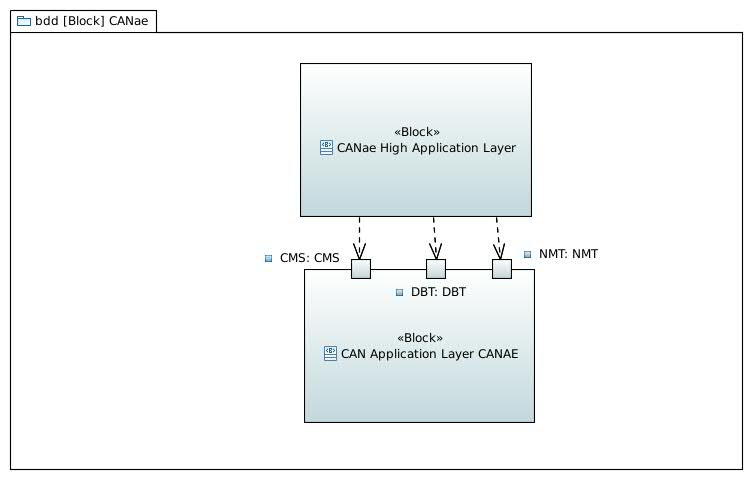
\includegraphics[scale=0.5]{images/Secciones/AppendixA/CANAE.JPG}
  \caption{Estructura de la capa de aplicación de CANae en alto nivel}
\label{fig:CANAEC4}
\end{figure}

Esto puede observar se en la Figura \ref{fig:CANAEC4}. En el gráfico se observa que
la CANae application Layer, cuenta con 3 interfaces:
\begin{itemize}
\item \textbf{CMS}: ofrece un ambiente orientado a objecto para diseñar aplicaciones de usuario.
  Esta entidad ofrece variables y eventos, y específica como un módulo pude acceder a
las interfaces de CAN.
\item \textbf{NMT}: ofrece un ambiente orientado a objetos para permitir que un módulo (el
NMT Master) se ocupe de la inicialización y posibles fallas de otros módulos (NMT Slaves).
\item \textbf{DBT}: ofrece el servicio para distribuir dinámicamente el identificador de para los diferentes nodos.
\end{itemize}
Debe destacarse que, el servicio CMS ofrece un ambiente orientado a objeto  para diseñar
aplicaciones de usuario, es decir, que ofrece la posibilidad de modelar el
comportamiento del sistema en forma de objeto. Este servicio ofrece la posibilidad
de crear variables y eventos, según las necesidades de los usuarios, que son
utilizadas para diseñar y especificar como la funcionalidad de un módulo puede
acceder a las interfaces de bajo nivel de CAN. Esto propone un grado de innovación
al tratar al protocolo, a los datos, mensajes y eventos como objetos, permitiendo así
un modelado orientado a objetos. Por tal motivo, este protocolo fue modelado
con SysML (System Modeling Language).
Para mayor detalle de estas interfaces se debe consultar en el apéndice \ref{Appendix:A}.

Agregando, dentro de esta capa existen dos entidades que juegan un papel importante
(consultar apéndice \ref{Appendix:A}) las cuales son:
\begin{itemize}
\item \textbf{Gestor de mensajes}: este se encarga de gestionar los mensajes que son enviados y recibidos desde la red.
Esta entidad debe ser capaz de determinar si el mensajes contiene datos o eventos. Trabaja en conjunto
con el CMS.
\item \textbf{Gestor de nodo}: esta entidad se encarga de llevar el control de los nodos existenten en la red. En este
nodo se encuentra la tabla de ruteo primario y secundario necesarios para la correcta comunicación.
\end{itemize}

La subcapa denominada CAN High Application Layer tiene una función más del lado de la gestión de nodos y tareas.
En esta capa se desarrollan los algoritmos necesarios para realizar el ruteo y la reconfiguración de la red ante
fallas, por lo tanto en la High Application Layer se debe implementar el sistema de FDIR. El protocolo no define ningún
algoritmo de ruteo, por lo que queda para el usuario la definición de los algoritmos.
El protocolo  recomienda desarrollar dos algoritmos, el primario y el secundario.
Para aumentar la tolerancia a fallas se pueden desarrollar más algoritmos
secundarios, y el switch entre algoritmos, puede depender de medidas de perfomance.

Así, queda conformada el protocolo de comunicación CANae como uno de los
principales productos de este trabajo de tesis. 
